\documentclass{article}
\usepackage{amsmath}
\usepackage{amsfonts}
\usepackage{amssymb}
\usepackage{hyperref}
\usepackage{graphicx}

\usepackage{theorem}

\usepackage{float}
\usepackage{booktabs}

\usepackage{algorithm,algpseudocode}
\usepackage{algorithm}

\usepackage{url}
\usepackage{caption}

\usepackage{listings}
\usepackage{color}

\definecolor{codegreen}{rgb}{0,0.6,0}
\definecolor{codegray}{rgb}{0.5,0.5,0.5}
\definecolor{codepurple}{rgb}{0.58,0,0.82}
\definecolor{backcolour}{rgb}{0.99,0.99,0.99}

\lstdefinestyle{mystyle}{
    backgroundcolor=\color{backcolour},   
    commentstyle=\color{codegreen},
    keywordstyle=\color{magenta},
    numberstyle=\tiny\color{codegray},
    stringstyle=\color{codepurple},
    basicstyle=\ttfamily\footnotesize,
    breakatwhitespace=false,         
    breaklines=true,                 
    captionpos=b,                    
    keepspaces=true,                 
    numbers=left,                    
    numbersep=5pt,                  
    showspaces=false,                
    showstringspaces=false,
    showtabs=false,                  
    tabsize=2
}

\usepackage[utf8]{inputenc}

\usepackage[backend=biber, style=authoryear, citestyle=authoryear]{biblatex}

\lstset{style=mystyle}

{
\title{
    \includegraphics[width=0.31\textwidth]{/Users/mlnick/documents/Logos_and_pics/TSUKUBA_logo.png} \\
    \vspace{3mm}
    \textbf{Transformer-Based Attacks on LWE} \\
    \vspace{3mm}    
    CryptoSemi proceeding
}

\author{Mamanchuk Mykola, SID.202420671}
\date{\today}

\begin{document}
\maketitle

\section{Introduction to the Concept}

\subsection{Importance of Lattice Cryptography}
Lattice cryptography has become a cornerstone in the development of post-quantum cryptographic protocols. Unlike classical cryptographic systems, which rely on the hardness of factoring large integers or computing discrete logarithms, lattice-based schemes are resistant to attacks by quantum computers. This resilience stems from the computational hardness of lattice problems, such as the Learning with Errors (LWE) problem, which remains intractable even for quantum algorithms.

The National Institute of Standards and Technology (NIST) has recognized the significance of lattice cryptography and has incorporated it into the standardization process for post-quantum cryptographic algorithms. Recent advancements in lattice cryptography include efficient algorithms for key exchange, encryption, and digital signatures, which provide strong security guarantees and practical performance.

\subsection{Introduction to SALSA}
The SALSA series of works marks a significant step in applying machine learning, specifically transformer models, to cryptographic attacks on lattice-based schemes. The initial hypothesis behind SALSA was that transformers, with their powerful sequence-to-sequence learning capabilities, could be effectively used to recover secrets from LWE instances. This innovative approach leverages the ability of transformers to model complex relationships within data, potentially uncovering patterns that traditional algorithms might miss.

The foundational work of SALSA set out to demonstrate the feasibility of this approach by applying it to LWE instances and comparing the results with traditional methods. The initial attempts faced several challenges, such as the need for extensive computational resources and the difficulty of training models on cryptographic data. Despite these challenges, the SALSA approach provided promising results, paving the way for further refinements in subsequent works like SALSA VERDE and SALSA PICANTE.

\section{Fundamentals of LWE}

\subsection{Learning with Errors (LWE) Problem}
The Learning with Errors (LWE) problem is a cornerstone of lattice-based cryptography, introduced by Oded Regev. The problem can be formulated as follows:

Given:
\begin{itemize}
    \item A secret vector \( s \in \mathbb{Z}_q^n \)
    \item A set of linear equations \( \mathbf{A} \mathbf{s} + \mathbf{e} \equiv \mathbf{b} \mod q \)
\end{itemize}

Where:
\begin{itemize}
    \item \( \mathbf{A} \in \mathbb{Z}_q^{m \times n} \) is a uniformly random matrix
    \item \( \mathbf{e} \in \mathbb{Z}_q^m \) is an error vector sampled from a probability distribution \( \chi \)
\end{itemize}

The objective is to recover the secret vector \( s \) given \( (\mathbf{A}, \mathbf{b}) \).

In a more detailed form, the LWE instances are expressed as:
\[ 
A_i \mathbf{s} + e_i \equiv b_i \mod q \quad \text{for} \quad i = 1, 2, \ldots, m
\]
where \( e_i \) is the error term.

\subsection{Binary and Ternary Secrets}
In LWE-based schemes, the secret key vector \( s \) can be sampled from various distributions for efficiency reasons. Common distributions include:
\begin{itemize}
    \item \textbf{Binary distributions}: \( s \in \{0, 1\}^n \)
    \item \textbf{Ternary distributions}: \( s \in \{-1, 0, 1\}^n \)
\end{itemize}

These distributions are especially useful in homomorphic encryption schemes, such as HEAAN, which typically use parameters like \( n = 2^{15} \), \( q = 2^{628} \), and ternary secrets with Hamming weight \( h \).

The Hamming weight of a binary or ternary secret refers to the number of non-zero elements in the vector. For example, a secret key of length 8 bits with a Hamming weight \( h = 3 \) can have 
\[
\frac{8!}{(8-3)!3!} = 56
\]
different keys. This can be visualized as:
\[ s_0 := 11100000 \]

While the exact Hamming weight \( h \) is typically not disclosed, a higher value introduces more noise, which can affect the efficiency of homomorphic schemes by making the bootstrapping process less efficient.

In the context of attacks like SALSA, a higher Hamming weight results in less efficient retrieval of the secret key due to the increased complexity and noise.

\subsection{Search-LWE and Decision-LWE}
The LWE problem comes in two main variants:
\begin{itemize}
    \item \textbf{Search-LWE}: The goal is to find the secret vector \( s \) given \( (\mathbf{A}, \mathbf{b}) \).
    \item \textbf{Decision-LWE}: The goal is to distinguish whether pairs \( (\mathbf{A}, \mathbf{b}) \) are sampled according to the LWE distribution or uniformly at random.
\end{itemize}

Regev's reduction shows that solving the Search-LWE problem is as hard as distinguishing LWE samples from random ones, establishing the foundational hardness of LWE.

\subsection{Applications and Importance}
LWE forms the basis for several cryptographic applications, including:
\begin{itemize}
    \item \textbf{Private-key and public-key encryption}: Secure schemes that ensure confidentiality and integrity of data.
    \item \textbf{Homomorphic encryption}: Allows computation on encrypted data without decryption.
    \item \textbf{Collision-resistant hashing}: Provides security against finding two different inputs that hash to the same output.
\end{itemize}

The security of these schemes is grounded in the hardness of the LWE problem, making it a critical area of study in post-quantum cryptography.

\subsection{Attacks on LWE}
Various attacks have been proposed to solve the LWE problem, exploiting different mathematical and computational techniques:
\begin{itemize}
    \item \textbf{Primal and dual lattice attacks}: Utilize lattice reduction algorithms to find short vectors that reveal the secret.
    \item \textbf{BKZ and LLL algorithms}: Advanced lattice reduction techniques used to improve the efficiency of attacks.
\end{itemize}

The SALSA series of works introduces transformer-based models as a novel approach to attacking LWE, showcasing the potential of machine learning in cryptographic research.

\section{LWE from the Perspective of Attacking with ML}

Two key factors make breaking LWE difficult: the presence of error and the use of modular arithmetic. Machine learning (ML) models tend to be robust to noise in their training data. In the absence of a modulus, recovering \( s \) from observations of \( a \) and \( b = a \cdot s + e \) merely requires linear regression, an easy task for ML. Once a modulus is introduced, attacking LWE requires performing linear regression on an \( n \)-dimensional torus, a much harder problem.

Modular arithmetic, therefore, appears to be a significant challenge for an ML-based attack on LWE. Previous research has concluded that modular arithmetic is difficult for ML models, and that transformers struggle with basic arithmetic. However, some studies showed that transformers can compute matrix-vector products, the basic operation in LWE, with high accuracy. As a first step towards attacking LWE, it is investigated whether these results can be extended to the modular case.

\subsection{Methods}

\textbf{Data Generation}: Training data is generated by fixing the modulus \( q \) (a prime with \( 15 \leq \lceil \log_2(q) \rceil \leq 30 \)), the dimension \( n \), and the secret \( s \in \mathbb{Z}_q^n \) (or \( \{0, 1\}^n \) in the binary case). Then, \( a \) is sampled uniformly in \( \mathbb{Z}_q^n \) and \( b = a \cdot s \mod q \) is computed, to create data pairs \( (a, b) \).

\textbf{Encoding}: Integers are encoded in base \( B \) (usually, \( B = 81 \)), as a sequence of digits in \( \{0, \ldots, B-1\} \). For instance, \( (a, b) = (16, 3) \) is represented as the sequences \([1,0,0,0,0]\) and \([1,1]\) in base 2, or \([2,2]\) and \([3]\) in base 7. In the multi-dimensional case, a special token separates the coordinates of \( a \).

\textbf{Model Training}: The model is trained to predict \( b \) from \( a \), for an unknown but fixed value of \( s \). Sequence-to-sequence transformers with one layer in the encoder and decoder, 512 dimensions, and 8 attention heads are used. Cross-entropy loss is minimized and the Adam optimizer with a learning rate of \( 5 \times 10^{-5} \) is employed. At epoch end (300,000 examples), model accuracy is evaluated over a test set of 10,000 examples. Training continues until test accuracy is 95\% or loss plateaus for 60 epochs.

\begin{table}[h]
    \centering
    \[
    \begin{array}{|c|c|c|c|c|c|c|c|c|c|}
    \hline
    \lceil \log_2(q) \rceil & 2 & 3 & 5 & 7 & 24 & 27 & 30 & 81 & 128 \\
    \hline
    15 & 23 & 21 & 23 & 22 & 20 & 23 & 22 & 20 & 20 \\
    16 & 24 & 22 & 22 & 22 & 22 & 22 & 22 & 22 & 21 \\
    17 & - & 23 & 25 & 22 & 23 & 24 & 22 & 22 & 22 \\
    18 & - & 23 & 25 & 23 & 23 & 24 & 25 & 22 & 22 \\
    19 & - & 23 & - & 25 & 25 & 24 & - & 25 & 24 \\
    20 & - & - & - & - & 24 & 25 & 24 & - & 25 \\
    21 & - & 24 & - & 25 & - & - & 25 & - & 25 \\
    22 & - & - & - & - & - & 25 & - & - & 25 \\
    23 & - & - & - & - & - & - & 25 & - & 25 \\
    \hline
    \end{array}
    \]
    \caption{Size of the training sets required for learning modular inversion. Base-2 logarithm of the number of examples needed to reach 95\% accuracy, for different values of \( \lceil \log_2(q) \rceil \) and bases. '-' means 95\% accuracy not attained after 90 million examples.}
    \end{table}
\textbf{Learning modular multiplication for various moduli}: The test loss and accuracy for \( q \) with \( \lceil \log_2(q) \rceil \) from 15 to 21, with 300,000 training examples/epoch, using one-layer transformers with 512 dimensions, 8 attention heads, integers encoded in base 81.

\[
\begin{array}{cc}
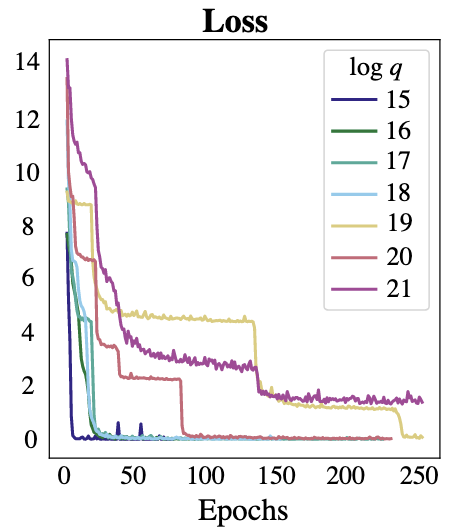
\includegraphics[width=0.4\textwidth]{loss.png} &
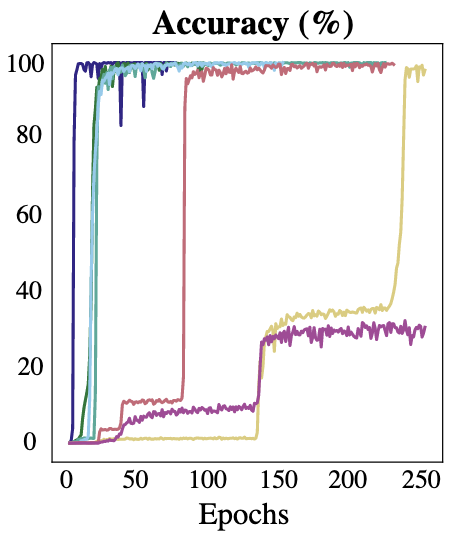
\includegraphics[width=0.4\textwidth]{accuracy.png} \\
\text{Figure 1: Test Loss} & \text{Figure 1: Test Accuracy}
\end{array}
\]

\textbf{Additional Experiments}: Additional information on model architecture is provided, specifically examining the effect of model layers, optimizer, embedding dimension, and batch size on integer modular inversion performance.

- Shallow transformers (e.g., 2 layers) work best, allowing to solve problems with a much higher \( q \) especially when the base \( B \) is large.
- The AdamCosine optimizer usually works best but requires smaller batch sizes for success with large bases.
- A smaller embedding dimension of 128 performs better, but increasing base size and dimension simultaneously yield good performance. Results on batch size do not show a strong trend.

\textbf{Base vs. Secret}

It is empirically observed that the base \( B \) used for integer representation in experiments may provide side-channel information about the secret \( s \) in the 1D case. For example, when the secret value is 729, bases 3, 9, 27, 729, and 3332 all enable solutions with much higher \( q \) (8 times higher than the next highest result). Nearly all these are powers of 3 as is the secret 729 \( = 3^6 \). In the table, one can see that these same bases provide similar (though not as significant) "boosts" in \( q \) for secrets on either side of 729 (e.g., 728, 730), as well as for 720 \( = 6^2 \).

Based on these results, it is speculated that when training on \( (a, b) \) pairs with an unknown secret \( s \), testing on different bases and observing model performance may allow some insight into \( s \)'s prime factors.

\subsection{Results for Recovering Secrets from Noisy Equations}

\textbf{One-Dimensional}: For a fixed secret \( s \), modular multiplication is a function from \( \mathbb{Z}_q \) into itself, that can be learned by memorizing \( q \) values. The models learn modular multiplication with high accuracy for values of \( q \) such that \( \lceil \log_2(q) \rceil \leq 22 \). Figure 1 presents learning curves for different values of \( \log_2(q) \). The loss and accuracy curves have a characteristic step shape, observed in many of our experiments, which suggests that "easier cases" (small values of \( \lceil as/q \rceil \)) are learned first.

The speed of learning and the training set size needed to reach high accuracy depend on the problem difficulty, i.e., the value of \( q \). Table 1 presents the \( \lceil \log_2 \rceil \) of the number of examples needed to reach 95\% accuracy for different values of \( \lceil \log_2(q) \rceil \) and base \( B \). Since transformers learn from scratch, without prior knowledge of numbers and moduli, this procedure is not data-efficient. The number of examples needed to learn modular multiplication is between \( 10q \) and \( 50q \). Yet, these experiments prove that transformers can solve the modular inversion problem in prime fields.

Table 1 illustrates an interesting point: learning difficulty depends on the base used to represent integers. For instance, base 2 and 5 allow the model to learn up to \( \lceil \log_2(q) \rceil = 17 \) and 18, whereas base 3 and 7 can reach \( \lceil \log_2(q) \rceil = 21 \). Larger bases, especially powers of small primes, enable faster learning. The relation between representation base and learning difficulty is difficult to explain from a number-theoretic standpoint.

\textbf{Multidimensional Random Integer Secrets}: In the \( n \)-dimensional case, the model must learn the modular dot product between vectors \( a \) and \( s \) in \( \mathbb{Z}_q^n \). This proves to be a much harder problem. For \( n = 2 \), with the same settings, small values of \( q \) (251, 367, and 967) can be learned with over 90\% accuracy, and \( q = 1471 \) with 30\% accuracy. In larger dimension, all models fail to learn with parameters tried so far. Increasing model depth to 2 or 4 layers, or dimension to 1024 or 2048 and attention heads to 12 and 16, improves data efficiency (less training samples are needed), but does not scale to larger values of \( q \) or \( n > 2 \).

\textbf{Multidimensional Binary Secrets}: Binary secrets make \( n \)-dimensional problems easier to learn. For \( n = 4 \), models solve problems with \( \lceil \log_2(q) \rceil \leq 29 \) with more than 99.5\% accuracy. For \( n = 6 \) and 8, cases \( \lceil \log_2(q) \rceil \leq 22 \) are solved with more than 85\% accuracy but do not achieve high accuracy for larger values of \( n \). Techniques for recovering secrets from a partially trained transformer are introduced. It is shown that these additional techniques allow recovery of sparse binary secrets for LWE instances with \( 30 \leq n \leq 128 \) (so far).

\textbf{Subconclusion:} These results highlight that, in the one-dimensional case, secret recovery can be learned relatively easily. In the case of multidimensional random integer secrets, the problem becomes significantly harder and less effective to solve with the current configuration. However, for multidimensional binary secrets, there is a drastic improvement in accuracy and performance, making it more efficient and convenient to use, particularly in applications of homomorphic cryptography.

\section{Introducing SALSA: LWE Cryptanalysis with Transformers}

Having established that transformers can perform integer modular arithmetic, this result is leveraged to propose SALSA, a method for \textbf{Secret-recovery Attacks on LWE via Seq2Seq models with Attention}.

\subsection{SALSA Ingredients}
SALSA has three modules: a transformer model \( \mathcal{M} \), a secret recovery algorithm, and a secret verification procedure. It is assumed that SALSA has access to a number of LWE instances in dimension \( n \) that use the same secret, i.e., pairs \((a, b)\) such that \( b = a \cdot s + e \mod q \), with \( e \) an error from a centered distribution with small standard deviation. SALSA runs in three steps. First, it uses LWE data to train \( \mathcal{M} \) to predict \( b \) given \( a \). Next, SALSA runs a secret recovery algorithm. It feeds \( \mathcal{M} \) special values of \( a \), and uses the output \( \tilde{b} = \mathcal{M}(a) \) to predict the secret. Finally, SALSA evaluates the guesses \( \tilde{s} \) by verifying that residuals \( r = b - a \cdot \tilde{s} \mod q \) computed from LWE samples have small standard deviation. If so, \( s \) is recovered and SALSA stops. If not, SALSA returns to step 1, and iterates.

\subsection{Model Training}
SALSA uses LWE instances to train a model that predicts \( b \) from \( a \) by minimizing the cross-entropy between the model prediction \( \tilde{b} \) and \( b \). The model architecture is a universal transformer [1], in which a shared transformer layer is iterated several times (the output from one iteration is the input to the next). The base model has two encoder layers, with 1024 dimensions and 32 attention heads, the second layer iterated 2 times, and two decoder layers with 512 dimensions and 8 heads, the second layer iterated 8 times. To limit computation in the shared layer, the copy-gate mechanism from [2] is used. Models are trained using the Adam optimizer with \( lr = 10^{-5} \) and 8000 warmup steps.

For inference, a beam search with depth 1 (greedy decoding) is utilized; at the end of each epoch, model accuracy over a test set of LWE samples is computed. Because of the error added when computing \( b = a \cdot s + e \), exact prediction of \( b \) is not possible. Therefore, accuracy within tolerance \( \tau (\text{acc}_\tau) \) is calculated: the proportion of predictions \( \tilde{b} = \mathcal{M}(a) \) that fall within \( \tau q \) of \( b \), i.e., such that \( \| b - \tilde{b} \| \leq \tau q \). In practice, \( \tau \) is set to 0.1.

\subsection{Secret Recovery}
Two algorithms are proposed for recovering \( s \): direct recovery from special values of \( a \), and distinguisher-based recovery using the binary search to decision reduction.

\subsubsection{Direct Secret Recovery}

The first technique, based on the LWE search problem, is analogous to a chosen plaintext attack. For each index \( i = 1, \ldots, n \), a guess of the \( i \)-th coordinate of \( s \) is made by feeding model \( \mathcal{M} \) the special value \( a_i = K e_i \) (all coordinates of \( e_i \) are 0 except the \( i \)-th), with \( K \) a large integer. If \( s_i = 0 \), and the model \( \mathcal{M} \) correctly approximates \( b_i = a_i \cdot s + e \) from \( a_i \), then we expect \( \tilde{b}_i := \mathcal{M}(a_i) \) to be a small integer since practically there is no \( a_i \cdot s \) in the equation while the model distinguishes such a property. Likewise, if \( s_i = 1 \), we expect a large integer. This technique is formalized in Algorithm 1.

\begin{algorithm}[H]
\caption{Direct Secret Recovery}
\begin{algorithmic}[1]
    \State \textbf{Input:} \( \mathcal{M}, K, n \)
    \State \textbf{Output:} secret \( s \)
    \State \( p = 0^n \)
    \For{\( i = 1, \ldots, n \)}
        \State \( a = 0^n \); \( a_i = K \)
        \State \( p_i = \mathcal{M}(a) \)
    \EndFor
    \State \Return \( s = \text{binarize}(p) \)
\end{algorithmic}
\end{algorithm}

\subsubsection{Distinguisher Secret Recovery}

The second algorithm for secret recovery is based on the decision-LWE problem. It uses the output of pretrained model \( \mathcal{M} \) to determine if LWE data \((a, b)\) can be distinguished from randomly generated pairs \((a_r, b_r)\). The algorithm for distinguisher-based secret recovery is shown in Algorithm 2.

The algorithm works as follows:

Suppose there are \( t \) LWE instances \((a, b)\) and \( t \) random instances \((a_r, b_r)\). For each secret coordinate \( s_i \), \( a \) is transformed into \( a'_i \) with:
\[ a'_{LWE}[:,i] = (a_{LWE}[:,i] + c) \mod q \]
where \( c \in \mathbb{Z}_q \) are random integers that correspond to the presence of random noise. The model \( \mathcal{M} \) is used to compute \( \mathcal{M}(a') \) and \( \mathcal{M}(a_r) \), obtaining predictions \( \tilde{B}_{LWE} \) and \( \tilde{B}_{unif} \). If the model has learned the secret and the \( i \)-th bit of \( s \) is 0, then \( \mathcal{M}(a') \) should be significantly closer to \( b \) than \( \mathcal{M}(a_r) \) is to \( b_r \).

The deviations are calculated as:
\[ dl = \left\| \tilde{B}_{LWE} - B_{LWE} \right\| \]
\[ du = \left\| \tilde{B}_{unif} - B_{unif} \right\| \]

For each \( dl[j] \) and \( du[j] \), the sum of true conditional expressions is counted:
\[ c_{LWE} = \sum \{1 \, | \, dl[j] < \text{bound}\} \]
\[ c_{unif} = \sum \{1 \, | \, du[j] < \text{bound}\} \]
where \( \text{bound} = q \cdot \tau \), \( q \) is the modulus used to generate the set, and \( \tau \) is a confidence parameter.

The final step checks if:
\[ c_{LWE} - c_{unif} \leq \text{acc}_{\tau} \cdot t / 2 \]
If true, then \( s_i = 1 \). If the deviation is more than the accuracy tolerance \( \text{acc}_{\tau} \cdot t / 2 \), it is assumed that the prediction is not close enough, and \( s = 0 \) can be used in place. Iterating on \( i \) allows recovery of the secret bit by bit. SALSA runs the distinguisher recovery algorithm when model \( \text{acc}_{\tau} = 0.1 \) is above 30\%. This is the theoretical limit for this approach to work.

The algorithm proposed in the work is provided in the Appendix A.

\subsection{Secret Verification}

At the end of the recovery step, we have 10 to 11 guesses \( \tilde{s} \) (depending on whether the distinguisher recovery algorithm was run). To verify them, we compute the residuals \( r = a \cdot \tilde{s} - b \mod q \) for a set of LWE samples \( (a, b) \). If \( s \) is correctly guessed, we have \( \tilde{s} = s \), so \( r = a \cdot s - b = e \mod q \) will be distributed as the error \( e \), with small standard deviation \( \sigma \). If \( \tilde{s} \neq s \), \( r \) will be (approximately) uniformly distributed over \( \mathbb{Z}_q \) (because \( a \cdot \tilde{s} \) and \( b \) are uniformly distributed over \( \mathbb{Z}_q \)), and will have standard deviation close to \( q / \sqrt{12} \). Therefore, we can verify if \( \tilde{s} \) is correct by calculating the standard deviation of the residuals: if it is close to \( \sigma \), the standard deviation of error, the secret was recovered. In the case that \( \sigma = 3 \) and \( q = 251 \), the standard deviation of \( r \) is around 3 if \( \tilde{s} = s \), and 72.5 if not.

\section{SALSA Evaluation}

In this section, presented experiments with SALSA. We generate datasets for LWE problems of different sizes, defined by the dimension and the sparsity of the binary secret. We use gated universal transformers, with two layers in the encoder and decoder. Default dimensions and attention heads in the encoder and decoder are 1024/512 and 16/4, but we vary them as we scale the problems. Models are trained on two NVIDIA Volta 32GB GPUs on an internal FAIR cluster.

\subsection{Data Generation}

The LWE data is randomly generated for SALSA training/evaluation given the following parameters: dimension \( n \), secret density \( d \), modulus \( q \), encoding base \( B \), binary secret \( s \), and error distribution \( \chi \). For this section, \( q = 251 \) and \( B = 81 \) are in use, fix the error distribution \( \chi \) to be a discrete Gaussian with \( \mu = 0, \sigma = 3 \), and randomly generate a binary secret \( s \).

Problem size \( n \) is varied (the LWE dimension) and the density \( d \) (the proportion of ones in the secret) to test attack success and to observe how it scales. For problem size, holds an experiment with \( n = 30 \) to \( n = 128 \). For density, experiment with \( 0.002 \leq d \leq 0.15 \). For a given \( n \), select \( d \) so that the Hamming weight of the binary secret (\( h = dn \)), is larger than 2. Data is generated using the RLWE variant of LWE, described in Appendix B. For RLWE problems, each \( a \) is one line of a circulant matrix generated from an initial vector \( \in \mathbb{Z}_q^n \). RLWE problems exhibit more structure than traditional LWE due to the use of the circulant matrix, which may help our models learn.

\textbf{Regarding RLWE parameter choices.} The choices of \( n, q, \) ring \( R, \) and error distribution determine the hardness of a given RLWE problem. In particular, prior works showed that many choices of polynomials defining the number ring \( R \) are provably weak when \( n \) is not a power of 2. Thus, mainly evaluate SALSA’s success against RLWE for cyclotomic rings with dimension \( n = 2^\ell \), \( \ell \in \{5, 6, 7\} \) (Table 2). However, to help understand how SALSA scales with \( n \), we also provide performance evaluations for \( n \) values that are not powers of 2, even though these RLWE settings may be subject to different attacks more efficient than SALSA.

\begin{table}[h]
    \centering
    \begin{tabular}{|c|c|c|c|}
    \hline
    Dim. \( n \) & Density \( d \) & \( \log_2 \) samples & Runtime (hours) \\
    \hline
    30 & 0.1 & 20.93 & 1.2 \\
    30 & 0.13 & 23.84 & 12.9 \\
    32 & 0.09 & 20.93 & 1.2 \\
    50 & 0.06 & 22.25 & 4.7 \\
    50 & 0.08 & 25.67 & 49.9 \\
    64 & 0.05 & 22.39 & 8 \\
    70 & 0.04 & 22.74 & 11.9 \\
    90 & 0.03 & 23.93 & 43.4 \\
    110 & 0.03 & 24.07 & 68.8 \\
    128 & 0.02 & 22.25 & 46.0 \\
    \hline
    \end{tabular}
    \caption{Full secret recovery. Highest density values at which the secret was recovered for each \( n, q = 251 \). The model has 1024/512 dimensions, 16/4 attention heads. (For \( n = 128 \), 1536/512 dimensions, 32/4 attention heads).}
    \end{table}
    

    \begin{figure}[!htp]
    \centering
    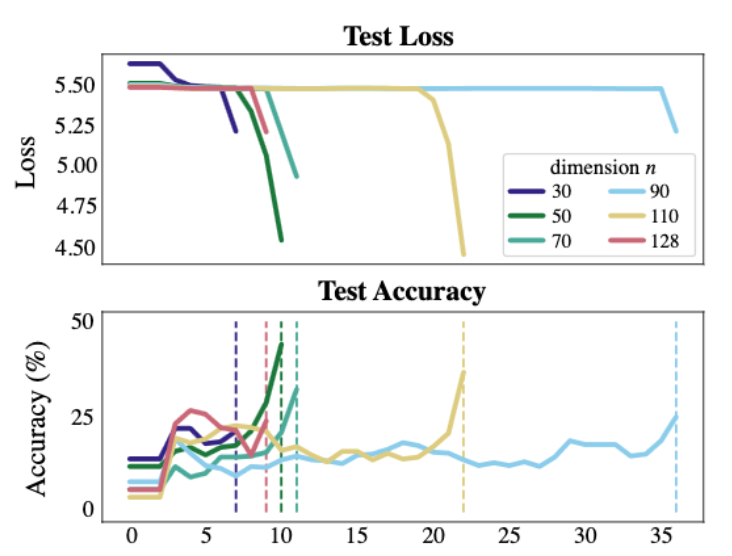
\includegraphics[width=0.8\textwidth]{fig2.png}
    \caption{(2) Full secret recovery: Curves for loss and \( \text{acc}_\tau = 0.1 \), for varying \( n \) with Hamming weight 3. For \( n < 100 \), model has 1024/512 embedding, 16/4 attention heads. For \( n \geq 100 \), model has 1536/512 embedding, 32/4 attention heads.}
    \end{figure}
    
    The figure on page 11 illustrates model behavior during training. After an initial burn-in period, the loss curve (top graph) plateaus until the model begins learning the secret. Once loss starts decreasing, model accuracy with 0.1q tolerance (bottom graph) increases sharply. Full secret recovery (vertical lines in the bottom graph) happens shortly after, often within one or two epochs. Direct secret recovery accounts for 55\% of recoveries, while the distinguisher only accounts for 18\% of recoveries. 27\% of the time, both methods succeed simultaneously.
    
    One key conclusion from these experiments is that the secret recovery algorithms enable secret recovery long before the transformer has been trained to high accuracy (even before training loss settles at a low level). Frequently, the model only needs to begin learning to achieve a successful revocery.    

\newpage

\section*{References}
\begin{enumerate}
    \item \textbf{Independent Research Group}, Universal Transformers, 2018. Available following arXiv library: \url{arXiv:1807.03819} [Accessed: 2024-05-12]
    \item \textbf{Semantic Scholar}, The Neural Data Router: Adaptive Control Flow in Transformers Improves Systematic Generalization, 2021. Available online: \url{https://www.semanticscholar.org/paper/The-Neural-Data-Router%3A-Adaptive-Control-Flow-in-Csord%C3%A1s-Irie/e528466e2aff981\\511d4ca6e063211297c0b4175} [Accessed: 2024-05-25]
    \item \textbf{University of Birmingham}, SALSA: Attacking Lattice Cryptography with Transformers, 2022. Available online: \url{https://eprint.iacr.org/2022/935.pdf} [Accessed: 2024-05-26]
    \item \textbf{Nicolas M., author himself}, Ongoing CryptoResearch, 2024. Available online: \href{https://www.petsourcing.com/wp-content/uploads/2018/11/How-to-Take-Care-of-Your-Cat-696x602.jpg}{https://docs.google.com/sheets/d/1LniEilwf\_e4lbKM\&sd=true} [La-st update: 2077-12-10]
\end{enumerate}

\newpage

\section*{Appendix A: Distinguisher Secret Recovery Algorithm}

\begin{algorithm}
    \caption{Distinguisher Secret Recovery}
    \begin{algorithmic}[1]
        \State \textbf{Input:} \( \mathcal{M}, n, q, \text{acc}_{\tau}, \tau \)
        \State \textbf{Output:} secret \( s \)
        \State \( s = 0^n \)
        \State \( \text{advantage}, \text{bound} = \text{acc}_{\tau} - 2 \cdot \tau, \tau \cdot q \)
        \State \( t = \min \left( 50, \frac{2}{\text{advantage}^2} \right) \)
        \State \( A_{LWE}, B_{LWE} = \text{LWE samples}(t, n, q) \)
        \For{\( i = 1, \ldots, n \)}
            \State \( A_{unif} \sim \mathbb{U}(0, q-1)^{n \times t} \)
            \State \( B_{unif} \sim \mathbb{U}(0, q-1)^t \)
            \State \( c \sim \mathbb{U}(0, q-1)^t \)
            \State \( A'_{LWE} = A_{LWE} \)
            \State \( A'_{LWE}[:,i] = (A_{LWE}[:,i] + c) \mod q \)
            \State \( \tilde{B}_{LWE} = \mathcal{M}(A'_{LWE}) \)
            \State \( \tilde{B}_{unif} = \mathcal{M}(A_{unif}) \)
            \State \( dl = \left\| \tilde{B}_{LWE} - B_{LWE} \right\| \)
            \State \( du = \left\| \tilde{B}_{unif} - B_{unif} \right\| \)
            \State \( c_{LWE} = \# \{ j \, | \, dl[j] < \text{bound}, j \in \mathbb{N}_t \} \)
            \State \( c_{unif} = \# \{ j \, | \, du[j] < \text{bound}, j \in \mathbb{N}_t \} \)
            \If{\( (c_{LWE} - c_{unif}) \leq \text{advantage} \cdot t / 2 \)}
                \State \( s_i = 1 \)
            \EndIf
        \EndFor
        \State \Return \( s \)
    \end{algorithmic}
    \end{algorithm}

    \newpage

    \section*{Appendix B: Further Details on LWE and Data Generation}
    \subsection*{Ring Learning with Errors}
    
    This section defines RLWE samples and explains how to generate LWE instances from them. Let \( n \) be a power of 2, and let \( R_q = \mathbb{Z}_q[x]/(x^n + 1) \) be the set of polynomials whose degrees are at most \( n-1 \) and coefficients are from \( \mathbb{Z}_q \). The set \( R_q \) forms a ring with additions and multiplications defined as the usual polynomial additions and multiplications in \( \mathbb{Z}_p[x] \) modulo \( x^n + 1 \). One RLWE sample refers to the pair 
    \[
    (a(x), b(x) := a(x) \cdot s(x) + e(x)),
    \]
    where \( s(x) \in R_q \) is the secret and \( e(x) \in R_q \) is the error with coefficients subject to the error distribution.
    
    Let \( a, s \) and \( e \in \mathbb{Z}_q^n \) be the coefficient vectors of \( a(x), s(x) \) and \( e(x) \). Then the coefficient vector \( b(x) \) of \( b(x) \) can be obtained via the formula
    \[
    b = A_{a(x)}^{\text{circ}} \cdot s + e,
    \]
    where \( A_{a(x)}^{\text{circ}} \) represents the \( n \times n \) generalized circulant matrix of \( a(x) \). Precisely, let \( a(x) = a_0 + a_1 x + \ldots + a_{n-2} x^{n-2} + a_{n-1} x^{n-1} \), then \( a = (a_0, a_1, \ldots, a_{n-2}, a_{n-1}) \) and 
    \[
    A_{a(x)}^{\text{circ}} =
    \begin{bmatrix}
    a_0 & -a_{n-1} & -a_{n-2} & \ldots & -a_1 \\
    a_1 & a_0 & -a_{n-1} & \ldots & -a_2 \\
    a_2 & a_1 & a_0 & \ldots & -a_3 \\
    \vdots & \vdots & \vdots & \ddots & \vdots \\
    a_{n-1} & a_{n-2} & a_{n-3} & \ldots & a_0 \\
    \end{bmatrix}.
    \]
    Therefore, one RLWE sample gives rise to \( n \) LWE instances by taking the rows of \( A_{a(x)}^{\text{circ}} \) and the corresponding entries in \( b \).
    
    \subsection*{Search to Decision Reduction for Binary Secrets}
    
    This section provides a proof of the search binary-LWE to decisional binary-LWE reduction. This is a simple adaptation of the reduction to the binary secrets case. An algorithm is called a \( (T, \gamma) \)-distinguisher for two probability distributions \( D_0, D_1 \) if it runs in time \( T \) and has a distinguishing advantage \( \gamma \). The notation \( \text{LWE}_{n,m,q,\chi} \) is used to denote the LWE problem which has secret dimension \( n \), \( m \) LWE instances, modulus \( q \) and the secret distribution \( \chi \).
    
    If there is a \( (T, \gamma) \)-distinguisher for decisional binary-LWE$_{n,m,q,\chi}$, then there is a \( T' = \tilde{O}(Tn/\gamma^2) \)-time algorithm that solves search binary-LWE$_{n,m',q,\chi}$ with probability \( 1 - o(1) \), where \( m' = \tilde{O}(m/\gamma^2) \).

    Let \( s = (s_1, \ldots, s_n) \) with \( s_i \in \{0, 1\} \). The strategy of recovering \( s_1 \), and the rest of the secret coordinates can be recovered in the same way. Let \( m' = \tilde{O}(1/\gamma^2)m \), given an LWE sample \( (A, b) \) where \( A \in \mathbb{Z}_q^{m' \times n}, b \in \mathbb{Z}_q^{m'} \), a pair \( (A', b') \) is computed as follows:
    \[
    A' = A + \mathbf{1}^T c, \quad b' = b.
    \]
    Here \( c \in \mathbb{Z}_q^{m'} \) is sampled uniformly and the symbol \( +\mathbf{1}^T \) indicates adding \( c \) to the first column of \( A \). The definition of LWE verifies that if \( s_1 = 0 \), then the pair \( (A', b') \) would be LWE samples with the same error distribution. Otherwise, the pair \( (A', b') \) would be uniformly random in \( \mathbb{Z}_q^{m' \times n} \times \mathbb{Z}_q^{m'} \). The pair \( (A', b') \) is then fed to the \( (T, \gamma) \)-distinguisher for LWE$_{n,m,q,\chi}$, running the distinguisher \( \tilde{O}(1/\gamma^2) \) times given the number of instances. If the majority of the outputs are “LWE”, then the pair \( (A', b') \) is an LWE sample and therefore \( s_1 = 0 \). If not, \( s_1 = 1 \).
    
    Guessing one coordinate requires running the distinguisher \( \tilde{O}(1/\gamma^2) \) times, thus the search to reduction algorithm takes time \( T' = \tilde{O}(Tn/\gamma^2) \). Note that the same \( m' \) LWE instances can be used for each coordinate, thus \( m' = \tilde{O}(m/\gamma^2) \) samples are required to recover all the secret coordinates.
    

\end{document}
